\section{Failure Analysis: The Limits of Prompting and Explicit Reasoning}
\label{sec:behavioral}

\begin{table*}[t]
\caption{Accuracy cost per saved call ($\frac{\Delta\text{Acc}}{-\Delta\text{TC}}$) when switching from Default~($\star$) to Sparse~(S). All changes are relative to Default (Prompt-only). More negative $\frac{\Delta\text{Acc}}{-\Delta\text{TC}}$ means each saved call costs more accuracy. Hard tasks pay a disproportionate price.}
\vspace{-5pt}
\label{tab:uniform_reduction}
\centering
\small
\setlength{\tabcolsep}{3pt}
\begin{tabular}{ll rrr rrr rrr}
\toprule
& & \multicolumn{3}{c}{Qwen3-4B-Inst.} & \multicolumn{3}{c}{Qwen3-14B} & \multicolumn{3}{c}{Llama-3.3-70B} \\
\cmidrule(lr){3-5} \cmidrule(lr){6-8} \cmidrule(lr){9-11}
Mode & Difficulty & $\Delta$Acc & $\Delta$TC & $\frac{\Delta\text{Acc}}{-\Delta\text{TC}}$ & $\Delta$Acc & $\Delta$TC & $\frac{\Delta\text{Acc}}{-\Delta\text{TC}}$ & $\Delta$Acc & $\Delta$TC & $\frac{\Delta\text{Acc}}{-\Delta\text{TC}}$ \\
\midrule
\multirow{3}{*}{Prompt-only}
  & Easy  & $-$14.5 & $-$0.84 & $-$17.3 & $-$8.8  & $-$0.59 & $-$14.9 & $+$1.6  & $-$0.51 & $+$3.2 \\
  & Medium& $-$20.7 & $-$0.86 & $-$24.1 & $-$12.9 & $-$0.53 & $-$24.3 & $+$2.0  & $-$0.41 & $+$4.8 \\
  & Hard  & $-$20.3 & $-$0.48 & $-$\textbf{42.4} & $-$27.3 & $-$0.47 & $-$\textbf{58.4} & $-$0.2  & $-$0.34 & $-$\textbf{0.5} \\
\midrule
\multirow{3}{*}{Reason-then-Act}
  & Easy  & $-$14.5 & $-$0.86 & $-$16.9 & $-$4.4  & $-$0.67 & $-$6.6  & $-$4.8  & $-$1.98 & $-$2.4 \\
  & Medium& $-$22.4 & $-$0.90 & $-$24.8 & $-$10.4 & $-$0.62 & $-$16.8 & $-$18.9 & $-$1.87 & $-$10.1 \\
  & Hard  & $-$13.0 & $-$0.35 & $-$\textbf{36.6} & $-$9.7  & $-$0.28 & $-$\textbf{34.7} & $-$63.3 & $-$1.99 & $-$\textbf{31.7} \\
\bottomrule
\end{tabular}
\end{table*}

\begin{figure}[t]
\centering
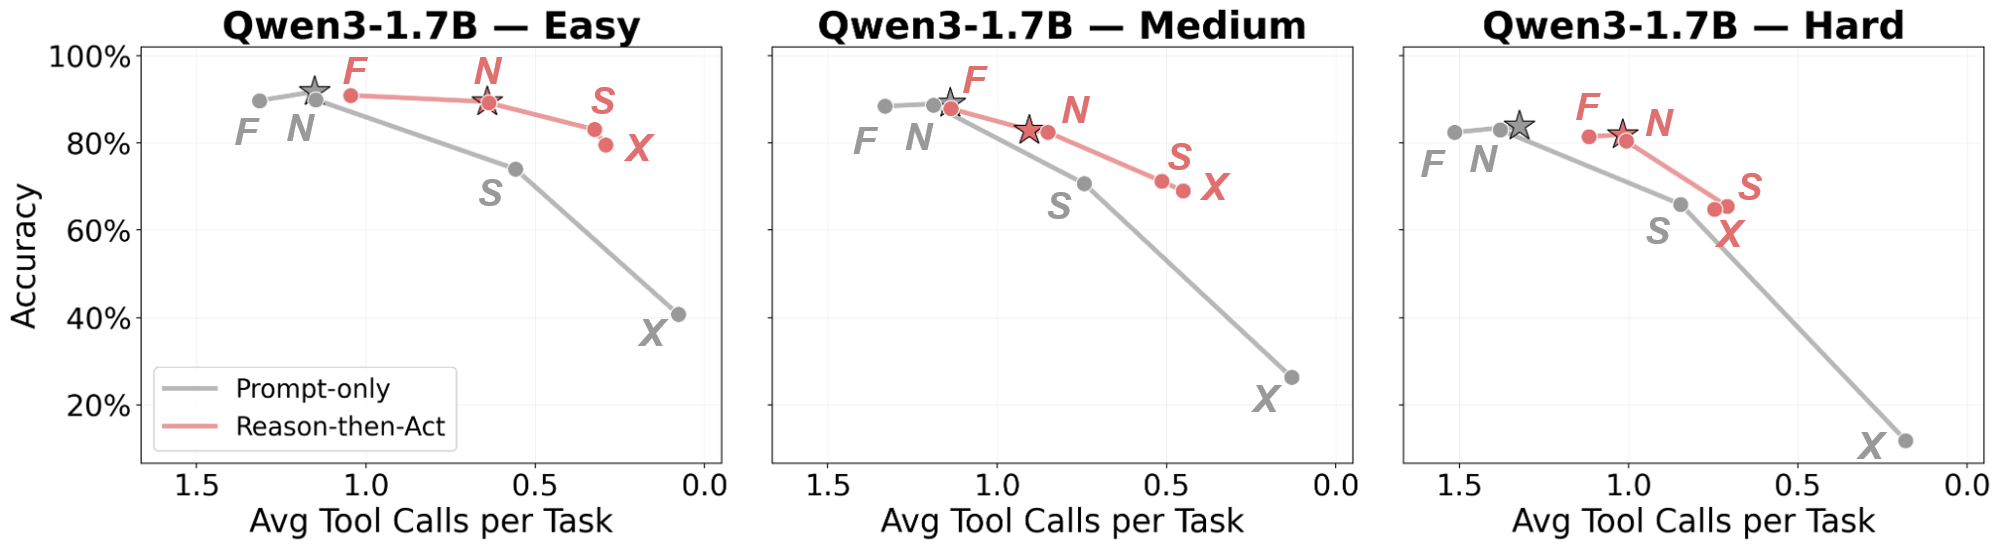
\includegraphics[width=\textwidth]{figures/fig3_baselines_manuallabel.png}
\vspace{-15pt}
\caption{Accuracy vs.\ Avg tool calls per difficulty for Qwen3-1.7B. $\star$=Default, F=Force, N=Necessary, S=Sparse, X=No~Tool. Reason-then-Act (red) partially shifts the tradeoff, reducing unnecessary easy-task calls, but still produces negative efficiency on hard tasks. Lines fold non-monotonically, reflecting coarse prompt control.}
\vspace{-10pt}
\label{fig:baselines}
\end{figure}

With \benchmark{} in place, we systematically test whether models can calibrate their tool usage through the two most natural training-free approaches: varying the prompt (Prompt-only) and asking the model to explicitly reason about tool necessity before acting (Reason-then-Act). Surprisingly, we found that these approaches based on prompt engineering and reasoning \textit{fail} to selectively reduce unnecessary tool calls as we show in the experiments. 

\subsection{Experimental setup}

We evaluate six models spanning two families: Qwen3-1.7B/4B/14B/32B and Llama-3.1-8B/3.3-70B. All experiments are run 3 times with different random seeds and we report mean results.

\paragraph{Prompt-only baselines.}
We test five prompt modes spanning the full range of tool-use instructions:
\textbf{Force~(F)}, ``tool use is mandatory'';
\textbf{Default~($\star$)}, no explicit requirements;
\textbf{Necessary~(N)}, ``only if necessary'';
\textbf{Sparse~(S)}, ``expensive, use sparingly'';
and \textbf{No~Tool~(X)}, ``do not use any tools.''

\paragraph{Reason-then-act baselines.}
In addition to prompt-only control, we evaluate a stronger baseline inspired by the think-before-act paradigm from ReAct~\citep{yao2022react} and Reflexion~\citep{shinn2023reflexion}. Before making a tool-call decision, the model is instructed to first reason about whether it can solve the task directly or needs a tool, then act on its own assessment. We apply this reasoning step to each of the same five prompt modes (Force, Default, Necessary, Sparse, No~Tool).

\subsection{Key findings}

\paragraph{Finding 1: Models default to tool overuse.}
Under the Default~($\star$) setting in Prompt-only baselines, models make 2,100--4,400 total tool calls across the 2,250-task single-hop test set, more than one calls per task. Even on easy tasks, Qwen3-1.7B makes 864 tool calls out of 750 easy tasks, and Llama-3.3-70B makes 1,482. The model's default behavior is ``tools are available, therefore use them,'' even when the task is simple enough to solve directly.
\vspace{-5pt}
\paragraph{Finding 2: Prompt engineering reduces tool calls indiscriminately, and hard tasks pay a disproportionate price.}
Prompts that discourage tool usage reduce calls across \emph{all} difficulty levels, including hard tasks where tools are genuinely needed. The reduction is far too indiscriminate: hard tasks lose substantially more accuracy per saved call than easy tasks. We quantify this with the \emph{accuracy cost per saved call}, $\frac{\Delta\text{Acc}}{-\Delta\text{TC}}$: how much accuracy is lost for each tool call eliminated. More negative means each saved call is more costly. Table~\ref{tab:uniform_reduction} shows this cost when moving from Default~($\star$) to Sparse~(S). On Qwen3-4B-Instruct, the cost is $-$17.3 on easy but reaches $-$42.4 on hard, meaning hard tasks lose 2.5$\times$ more accuracy per saved call. This pattern holds across model sizes.
\vspace{-5pt}
\paragraph{Finding 3: Reason-then-Act only partially helps, but with additional cost.}
Reasoning before decisions partially mitigates this problem: the accuracy cost per saved call improves on easy tasks (e.g., Qwen3-14B easy improves from $-$14.9 to $-$6.6 in Table~\ref{tab:uniform_reduction}). Figure~\ref{fig:baselines} shows Reason-then-Act (red lines) sits closer to the upper-right region on easy tasks, indicating that reasoning does reduce some unnecessary calls. However, reasoning still carries a high accuracy cost per saved call on hard tasks (e.g., $-$34.7 for Qwen3-14B), since it also suppresses tool calls where they are genuinely needed. Critically, this partial improvement comes at a cost: reasoning requires the model to generate additional tokens, increasing the generation overhead. Moreover, reasoning is model-dependent: on Llama-3.1-8B, accuracy drops from 79.5\% to 31.2\%; on Llama-3.3-70B, from 83.1\% to 47.9\%, as the model narrates its intent to call tools but never produces a valid invocation, resulting in near-zero tool calls (see Table~\ref{tab:singlehop_full} in Appendix~\ref{app:full_reduction} for full details).
\vspace{-5pt}
\paragraph{Finding 4: Prompt engineering cannot precisely control the accuracy--tool-call tradeoff.}
In practice, a user may want to set a tool-call budget and maximize accuracy under that budget. Figure~\ref{fig:baselines} shows that neither Prompt-Only nor Reason-then-Act can achieve this: each prompt mode provides a single, fixed operating point, with no way to smoothly adjust the tradeoff. Furthermore, many of these operating points are nearly indistinguishable: instructing the model to use tools ``only if necessary'' (N) produces almost identical behavior to the neutral Default~($\star$), while in Reason-then-Act mode, Sparse~(S) and No~Tool~(X) collapse to nearly the same point. The two baselines offer only a few effective operating points, making it impossible to precisely target a desired budget.


These findings establish that prompt-level control over tool-call decisions is limited, coarse, and unreliable across models. The models appear to lack the ability to translate task understanding into calibrated tool-call decisions through the generation process. This raises the question: is the model \emph{unable} to assess tool necessity, or does it know internally but fail to act on it? We investigate this in the next section.

